\documentclass[a4paper,14pt]{extarticle}

\usepackage[a4paper,top=20mm,bottom=20mm,left=30mm,right=10mm]{geometry}
\usepackage[T1,T2A]{fontenc}
\usepackage[utf8]{inputenc}
\usepackage[russian]{babel}
\usepackage{indentfirst}
\usepackage{titlesec}
\usepackage{graphicx}
\usepackage{verbatim}
\usepackage{fancyvrb}

\renewcommand{\baselinestretch}{1.3}
\titleformat{\section}{\normalsize\bfseries}{\thesection}{1em}{}
\titleformat{\subsection}{\normalsize\bfseries}{\thesection}{1em}{}
\setlength{\parindent}{12.5mm}

\begin{document}

  \newpage\thispagestyle{empty}
  \begin{center}
    \MakeUppercase{
      Министерство науки и высшего образования Российской Федерации\\
      Федеральное государственное бюджетное образовательное учреждение высшего образования\\
      <<Вятский Государственный Университет>>\\
    }
    Институт математики и информационных систем\\
    Факультет автоматики и вычислительной техники\\
    Кафедра электронных вычислительных машин
  \end{center}
  \vfill

  \begin{center}
    Отчет по лабораторной работе №4\\
    по дисциплине\\
    <<Управление данными>>\\
  \end{center}
  \vfill

  \noindent
  \begin{tabular}{ll}
    Выполнил студент гр. ИВТб-2301-05-00 \hspace{5mm} &
    \rule[-1mm]{25mm}{0.10mm}\,/Макаров С.А./\\
    
    Преподаватель & \rule[-1mm]{25mm}{0.10mm}\,/Клюкин В.Л./\\
  \end{tabular}

  \vfill
  \begin{center}
    Киров 2025
  \end{center}

  \newpage
  \section*{Цель}
  Цель лабораторной работы: познакомиться c библиотекой в C для связывания приложения с БД, изучить некоторые шаблоны проектирования, связанные с работой с БД, освоить на практике основы взаимодействия с БД под управлением PostgreSQL в приложении на C.

  \section*{Задание}
  При выполнении работы нужно использовать БД, созданную в предыдущих лабораторных работах. Необходимо создать приложение на языке программирования С с графическим интерфейсом.

  Требования к интерфейсу:
  \begin{itemize}
    \item[--] Названия колонок, кнопок, объектов ввода/вывода на русском языке (Например, ‘Имя’, а не ‘Name’),
    \item[--] Запретить ввод отрицательных значений (Например, цена не может быть отрицательной),
    \item[--] Ввод данных для выборки должен быть регистронезависимый (используйте функции UPPER или LOWER),
    \item[--] Для ввода даты, по возможности, использовать календарь.
  \end{itemize}

  Для любой одной таблицы, которая содержит внешний ключ на другую таблицу, приложение должно выполнять следующие функции:
  \begin{itemize}
    \item[--] Выводить, удалять и изменять данные таблицы,
    \item[--] В случае ввода уже имеющихся данных выводить сообщение об этом пользователю без записи данных в таблицу,
    \item[--] Удалять при подтверждении (Например, ‘Вы действительно уверены?’ Да/Нет),
    \item[--] Выполнять фильтр (выборку) по значениям строк. (Например, «Дата с … по …» или «Имя содержит …»).
  \end{itemize}

  Требования к реализации:
  \begin{itemize}
    \item[--] При добавлении новой строки внешний ключ выбирается из списка значений родительской таблицы (например, если таблица «Чек» ссылается на таблицу «Товар», нужно вывести список не id товара, а его название),
    \item[--] Сохранение или удаление строки должно быть реализовано с помощью функции PL/pgSQL
    \item[--] Фильтрация значений при поиске должна производиться через запрос, а не в полученной коллекции
    \item[--] Разрешается использование любого фреймворка,
    \item[--] При разработке можно использовать шаблоны проектирования, связанные с работой с БД
  \end{itemize}

  \pagebreak
  \section*{Решение}

  \begin{figure}[h]
    \centering
    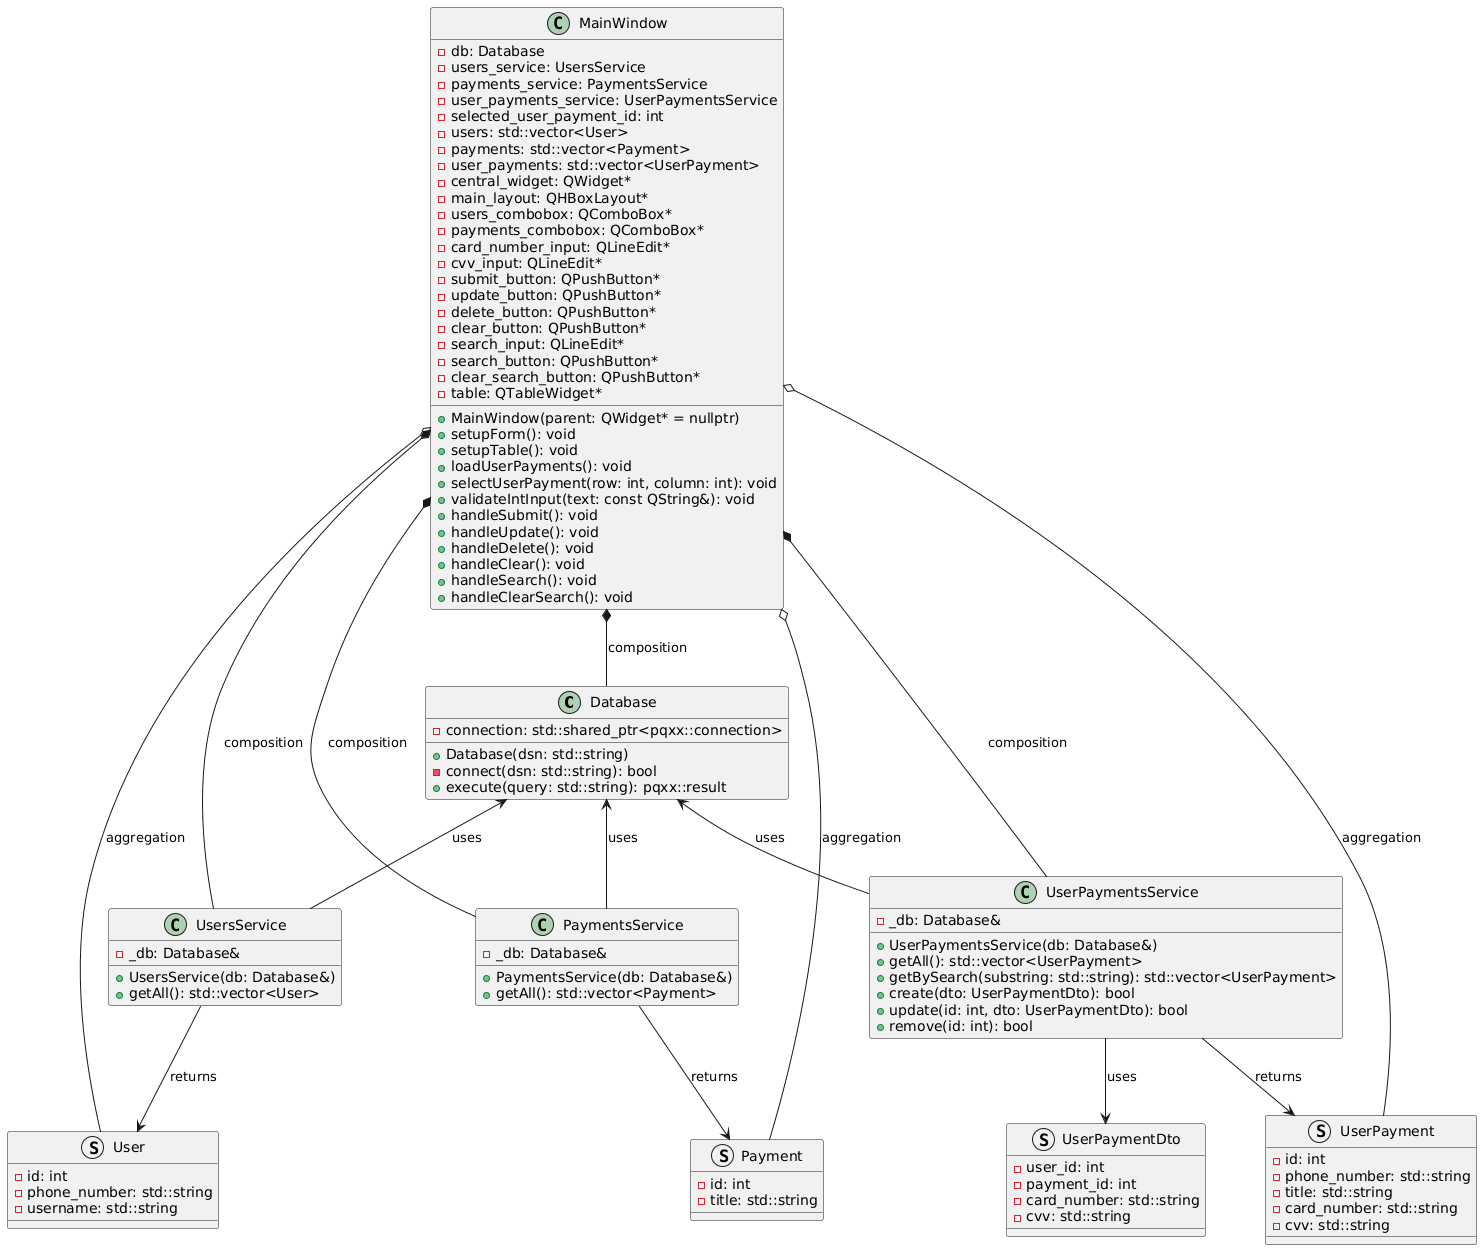
\includegraphics[width=1\linewidth]{img/uml-cpp.png}
  \end{figure}
  \begin{center}
    Рисунок 1 – Диаграмма классов
  \end{center}

  \pagebreak
  \begin{figure}[h]
    \centering
    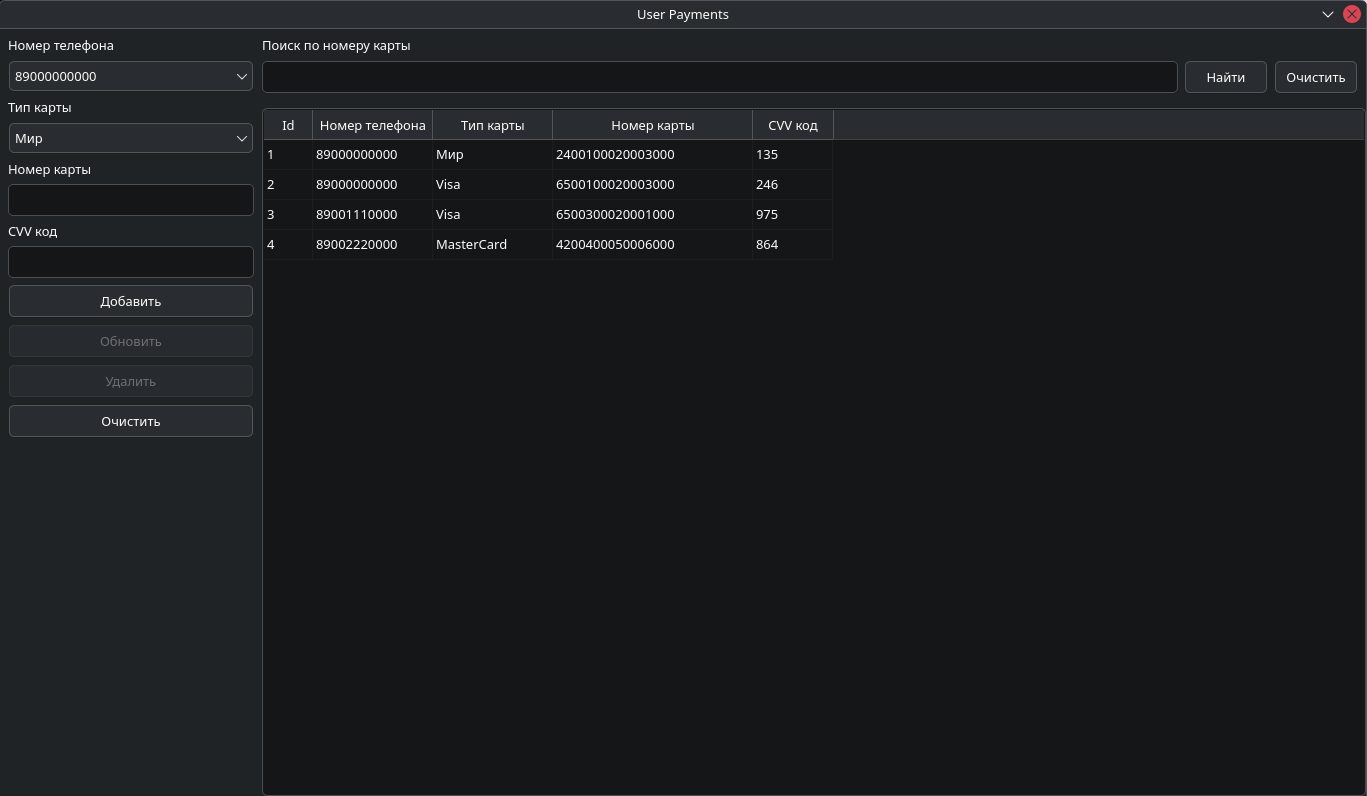
\includegraphics[width=0.95\linewidth]{img/f-1}
  \end{figure}
  \begin{center}
    Рисунок 2 – Форма таблицы способов оплаты пользователя
  \end{center}

  \begin{figure}[h]
    \centering
    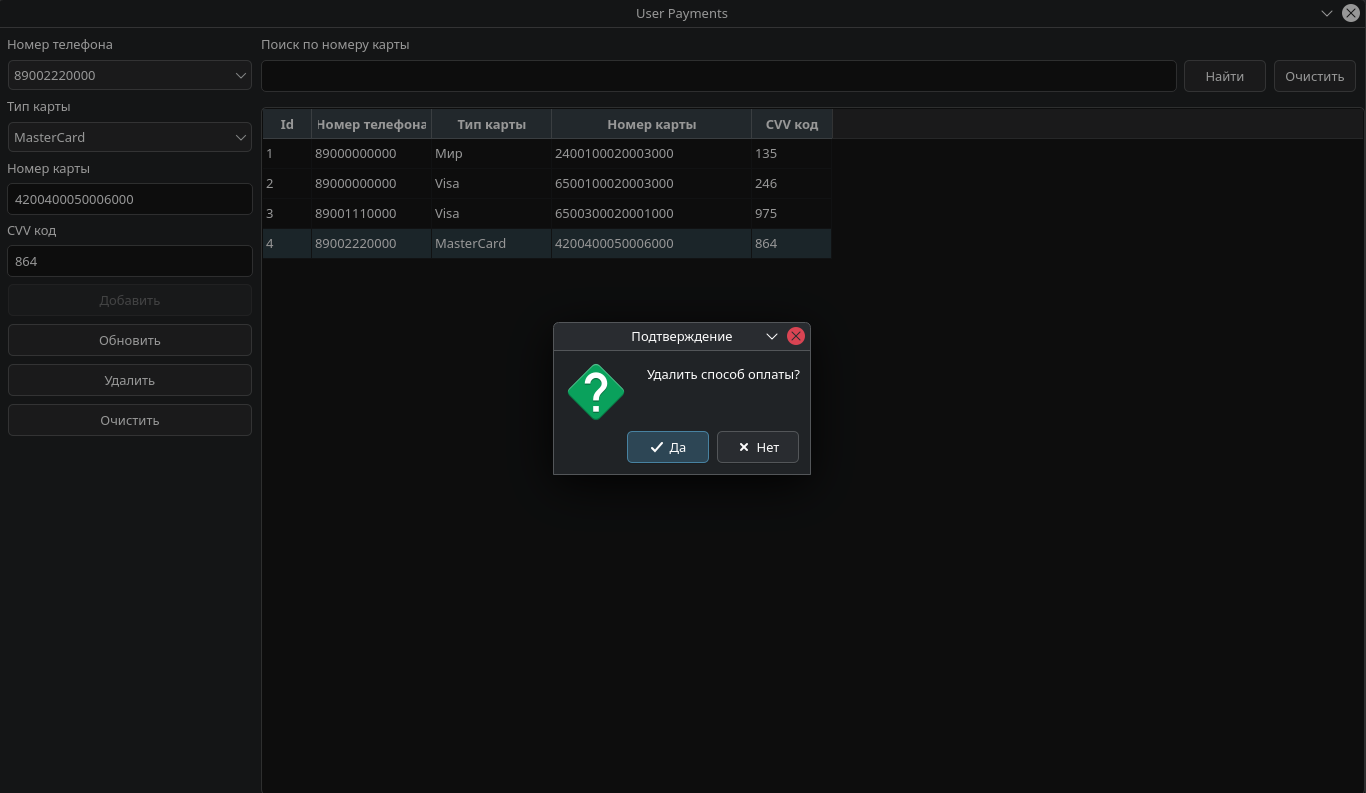
\includegraphics[width=0.95\linewidth]{img/f-2}
  \end{figure}
  \begin{center}
    Рисунок 3 – Подтверждение удаления записи
  \end{center}

  \pagebreak
  \begin{figure}[h]
    \centering
    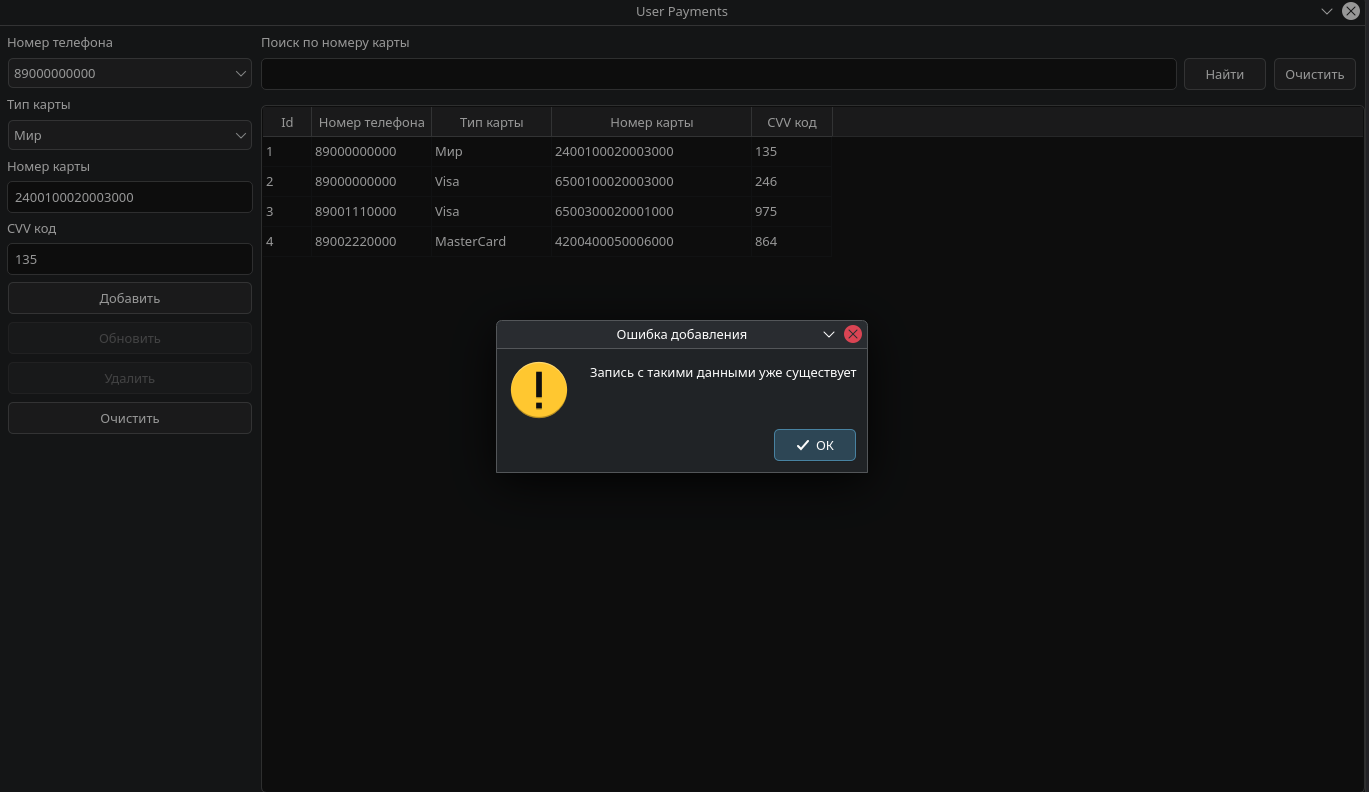
\includegraphics[width=0.95\linewidth]{img/f-3}
  \end{figure}
  \begin{center}
    Рисунок 4 – Сообщение при добавлении существующей записи
  \end{center}

  \begin{figure}[h]
    \centering
    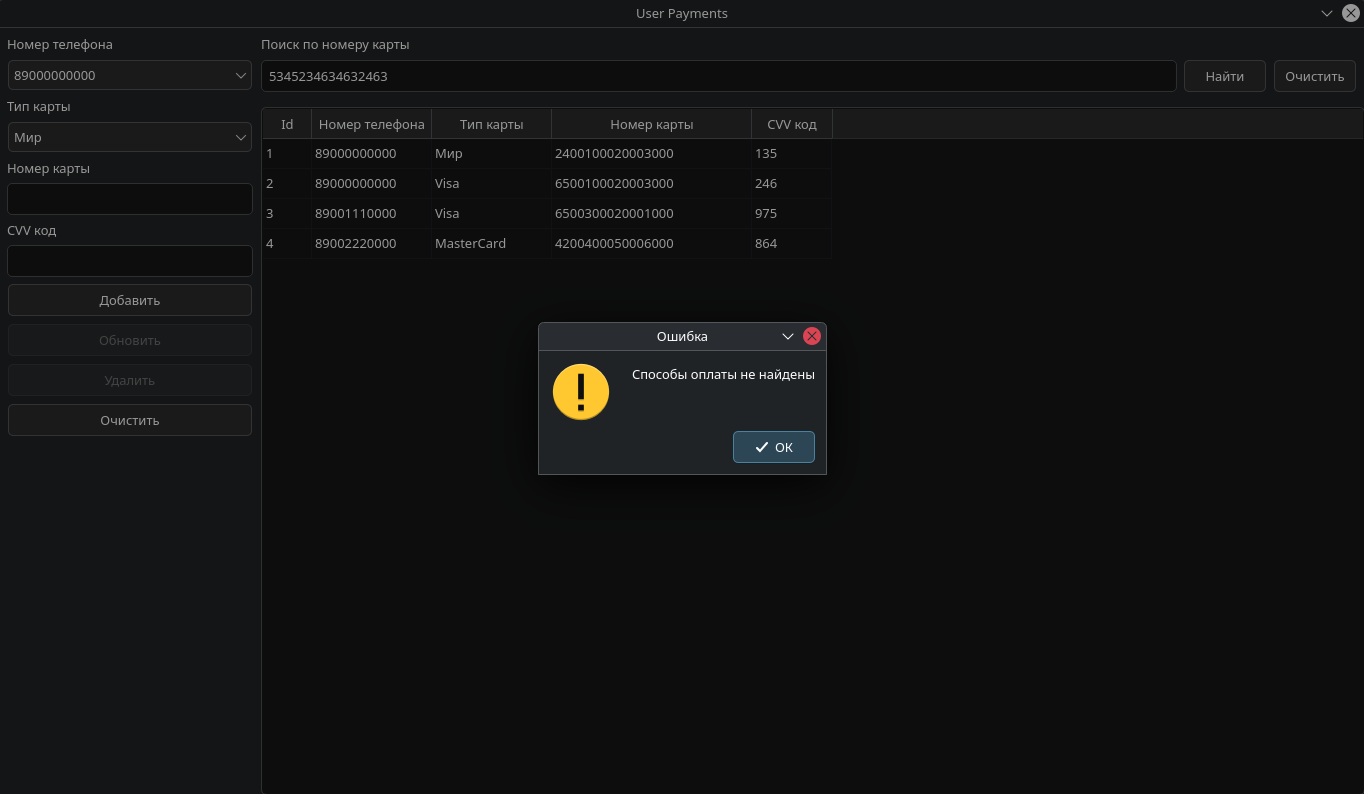
\includegraphics[width=0.95\linewidth]{img/f-4}
  \end{figure}
  \begin{center}
    Рисунок 5 – Сообщение при не найденных записях
  \end{center}

  \noindent
  \begin{Verbatim}[tabsize=4,fontsize=\small]
#include "windows/main_window.h"

#include <QApplication>

int main(int argc, char *argv[])
{
    QApplication app(argc, argv);    

    MainWindow window;
    window.show();

    return app.exec();
}

#pragma once

#include <pqxx/pqxx>
#include <string>

class Database
{
private:
    std::shared_ptr<pqxx::connection> connection;

    bool connect(std::string dsn);

public:
    Database(std::string dsn);

    pqxx::result execute(std::string query);
};

#include "database.h"

#include <iostream>

Database::Database(std::string dsn)
{
    Database::connect(dsn);
}

bool Database::connect(std::string dsn)
{
    try
    {
        connection = std::make_shared<pqxx::connection>(dsn);

        if (connection->is_open()) {
            std::cout << "Connected to database: " << connection->dbname() 
                                                  << std::endl;

            return true;
        } else {
            std::cout << "Failed to connect to database: " << dsn << std::endl;

            return false;
        }
    }
    catch(const std::exception& e)
    {
        std::cerr << "Database connection error: " << e.what() << std::endl;

        return false;
    }
}

pqxx::result Database::execute(const std::string query)
{
    try
    {
        pqxx::work txn(*connection);

        auto result = txn.exec(query);

        txn.commit();

        return result;
    }
    catch(const std::exception& e)
    {
        std::cerr << "Query execution error: " << e.what() << std::endl;
    }
}

#include "../database/database.h"

#include <string>
#include <vector>
#include <iostream>

struct User
{
    int id;
    std::string phone_number;
    std::string username;
};

class UsersService
{
private:
    Database &_db;

public:
    UsersService(Database &db);

    std::vector<User> getAll();
};

#include "users_service.h"

UsersService::UsersService(Database &db) : _db(db) {}

std::vector<User> UsersService::getAll()
{
    std::vector<User> users;

    try
    {
        pqxx::result result = _db.execute("SELECT * FROM users");

        for (const auto& row : result) {
            User user;

            user.id = row[0].as<int>();
            user.phone_number = row[1].as<std::string>();
            user.username = row[2].as<std::string>();

            users.push_back(user);
        }
    }
    catch(const std::exception& e)
    {
        std::cerr << "Get all users error: " << e.what() << std::endl;
    }

    return users;
}

#include "../database/database.h"

#include <string>
#include <vector>
#include <iostream>

struct Payment
{
    int id;
    std::string title;
};

class PaymentsService
{
private:
    Database &_db;

public:
    PaymentsService(Database &db);

    std::vector<Payment> getAll();
};

#include "payments_service.h"

PaymentsService::PaymentsService(Database &db) : _db(db) {}

std::vector<Payment> PaymentsService::getAll()
{
    std::vector<Payment> payments;

    try
    {
        pqxx::result result = _db.execute("SELECT * FROM payments");

        for (const auto& row : result) {
            Payment payment;

            payment.id = row[0].as<int>();
            payment.title = row[1].as<std::string>();

            payments.push_back(payment);
        }
    }
    catch(const std::exception& e)
    {
        std::cerr << "Get all payments error: " << e.what() << std::endl;
    }

    return payments;
}

#include "../database/database.h"

#include <string>
#include <format>
#include <vector>
#include <iostream>

struct UserPayment
{
    int id;
    std::string phone_number;
    std::string title;
    std::string card_number;
    std::string cvv;
};

struct UserPaymentDto
{
    int user_id;
    int payment_id;
    std::string card_number;
    std::string cvv;
};

class UserPaymentsService
{
private:
    Database &_db;

public:
    UserPaymentsService(Database &db);

    std::vector<UserPayment> getAll();
    std::vector<UserPayment> getBySearch(const std::string substring);
    bool create(UserPaymentDto dto);
    bool update(int id, UserPaymentDto dto);
    bool remove(int id);
};

#include "user_payments_service.h"

UserPaymentsService::UserPaymentsService(Database &db) : _db(db) {}

std::vector<UserPayment> UserPaymentsService::getAll()
{
    std::vector<UserPayment> user_payments;

    try
    {
        pqxx::result result = _db.execute(
            "SELECT up.id, u.phone_number, p.title, up.card_number, up.cvv "
            "FROM user_payments up "
                "JOIN users u ON u.id = up.user_id "
                "JOIN payments p ON p.id = up.payment_id"
        );

        for (const auto& row : result) {
            UserPayment user_payment;

            user_payment.id = row[0].as<int>();
            user_payment.phone_number = row[1].as<std::string>();
            user_payment.title = row[2].as<std::string>();
            user_payment.card_number = row[3].as<std::string>();
            user_payment.cvv = row[4].as<std::string>();

            user_payments.push_back(user_payment);
        }
    }
    catch(const std::exception& e)
    {
        std::cerr << "Get all user payments error: " << e.what() << std::endl;
    }

    return user_payments;
}

std::vector<UserPayment> UserPaymentsService::getBySearch(
  const std::string substring
)
{
    std::vector<UserPayment> user_payments;

    try
    {
        pqxx::result result = _db.execute(
            "SELECT up.id, u.phone_number, p.title, up.card_number, up.cvv "
            "FROM user_payments up "
                "JOIN users u ON u.id = up.user_id "
                "JOIN payments p ON p.id = up.payment_id "
            "WHERE up.card_number LIKE '%" + substring + "%'"
        );

        for (const auto& row : result) {
            UserPayment user_payment;

            user_payment.id = row[0].as<int>();
            user_payment.phone_number = row[1].as<std::string>();
            user_payment.title = row[2].as<std::string>();
            user_payment.card_number = row[3].as<std::string>();
            user_payment.cvv = row[4].as<std::string>();

            user_payments.push_back(user_payment);
        }
    }
    catch(const std::exception& e)
    {
        std::cerr << "Get user payments by search error: " 
                  << e.what() << std::endl;
    }

    return user_payments;
}

bool UserPaymentsService::create(UserPaymentDto dto)
{
    try
    {
        _db.execute(
            std::format(
                "SELECT create_user_payment({}, {}, '{}', '{}')",
                dto.user_id, dto.payment_id, dto.card_number, dto.cvv
            )
        );

        return true;
    }
    catch(const std::exception& e)
    {
        std::cerr << "Create user payments error: " << e.what() << std::endl;

        return false;
    }
}

bool UserPaymentsService::update(int id, UserPaymentDto dto)
{
    try
    {
        _db.execute(
            std::format(
                "SELECT update_user_payment({}, {}, {}, '{}', '{}')",
                id, dto.user_id, dto.payment_id, dto.card_number, dto.cvv
            )
        );

        return true;
    }
    catch(const std::exception& e)
    {
        std::cerr << "Update user payments error: " << e.what() << std::endl;

        return false;
    }
}

bool UserPaymentsService::remove(int id)
{
    try
    {
        _db.execute(
            std::format(
                "DELETE FROM user_payments WHERE id = {}", id
            )
        );

        return true;
    }
    catch(const std::exception& e)
    {
        std::cerr << "Delete user payments error: " << e.what() << std::endl;

        return false;
    }
}

#include "../services/users_service.h"
#include "../services/payments_service.h"
#include "../services/user_payments_service.h"

#include <vector>

#include <QApplication>
#include <QMainWindow>
#include <QWidget>
#include <QVBoxLayout>
#include <QHBoxLayout>
#include <QLabel>
#include <QLineEdit>
#include <QComboBox>
#include <QPushButton>
#include <QTableWidget>
#include <QTableWidgetItem>
#include <QHeaderView>
#include <QMessageBox>

class MainWindow : public QMainWindow
{
private:
    Database db;

    UsersService users_service;
    PaymentsService payments_service;
    UserPaymentsService user_payments_service;

    int selected_user_payment_id;

    std::vector<User> users;
    std::vector<Payment> payments;
    std::vector<UserPayment> user_payments;

    QWidget *central_widget;
    QHBoxLayout *main_layout;

    QComboBox *users_combobox;
    QComboBox *payments_combobox;
    QLineEdit *card_number_input;
    QLineEdit *cvv_input;
    QPushButton *submit_button;
    QPushButton *update_button;
    QPushButton *delete_button;
    QPushButton *clear_button;

    QLineEdit *search_input;
    QPushButton *search_button;
    QPushButton *clear_search_button;
    QTableWidget *table;

private slots:
    void validateIntInput(const QString &text);

public:
    MainWindow(QWidget *parent = nullptr);

    void setupForm();
    void setupTable();

    void loadUserPayments();
    void selectUserPayment(int row, int column);

    void handleSubmit();
    void handleUpdate();
    void handleDelete();
    void handleClear();
    void handleSearch();
    void handleClearSearch();
};

#include "main_window.h"

MainWindow::MainWindow(QWidget *parent)
    : QMainWindow(parent)
    , db("dbname=dm_db user=root password=root host=localhost port=5432")
    , users_service(db)
    , payments_service(db)
    , user_payments_service(db)
{
    central_widget = new QWidget();

    main_layout = new QHBoxLayout(central_widget);
    main_layout->setContentsMargins(0, 0, 0, 0);
    main_layout->addSpacing(0);

    setWindowTitle("User Payments");
    setFixedSize(1366, 768);
    setCentralWidget(central_widget);

    users = users_service.getAll();
    payments = payments_service.getAll();
    user_payments = user_payments_service.getAll();

    MainWindow::setupForm();
    MainWindow::setupTable();

    MainWindow::loadUserPayments();
}

void MainWindow::setupForm()
{
    QVBoxLayout *form_layout = new QVBoxLayout();

    form_layout->setContentsMargins(8, 8, 2, 8);
    form_layout->addSpacing(0);
    form_layout->setAlignment(Qt::AlignTop);

    users_combobox = new QComboBox();
    
    for (const auto& user : users) {
        users_combobox->addItem(
          QString::fromStdString(user.phone_number), user.id
        );
    }

    payments_combobox = new QComboBox();

    for (const auto& payment : payments) {
        payments_combobox->addItem(
          QString::fromStdString(payment.title), payment.id
        );
    }

    card_number_input = new QLineEdit();
    card_number_input->setMaxLength(16);
    connect(
      card_number_input, &QLineEdit::textChanged, this,
      &MainWindow::validateIntInput
    );

    cvv_input = new QLineEdit();
    cvv_input->setMaxLength(3);
    connect(
      cvv_input, &QLineEdit::textChanged, this, &MainWindow::validateIntInput
    );

    submit_button = new QPushButton("Добавить");
    connect(
      submit_button, &QPushButton::clicked, this, &MainWindow::handleSubmit
    );

    update_button = new QPushButton("Обновить");
    update_button->setEnabled(false);
    connect(
      update_button, &QPushButton::clicked, this, &MainWindow::handleUpdate
    );

    delete_button = new QPushButton("Удалить");
    delete_button->setEnabled(false);
    connect(
      delete_button, &QPushButton::clicked, this, &MainWindow::handleDelete
    );

    clear_button = new QPushButton("Очистить");
    connect(
      clear_button, &QPushButton::clicked, this, &MainWindow::handleClear
    );

    form_layout->addWidget(new QLabel("Номер телефона"));
    form_layout->addWidget(users_combobox);
    form_layout->addWidget(new QLabel("Тип карты"));
    form_layout->addWidget(payments_combobox);
    form_layout->addWidget(new QLabel("Номер карты"));
    form_layout->addWidget(card_number_input);
    form_layout->addWidget(new QLabel("CVV код"));
    form_layout->addWidget(cvv_input);
    
    form_layout->addWidget(submit_button);
    form_layout->addWidget(update_button);
    form_layout->addWidget(delete_button);
    form_layout->addWidget(clear_button);

    QWidget *form_container = new QWidget();
    form_container->setFixedWidth(256);
    form_container->setLayout(form_layout);

    main_layout->addWidget(form_container);
}

void MainWindow::setupTable()
{
    search_input = new QLineEdit();
    search_input->setMaxLength(16);
    connect(
      search_input, &QLineEdit::textChanged, this,
      &MainWindow::validateIntInput
    );

    search_button = new QPushButton("Найти");
    connect(
      search_button, &QPushButton::clicked, this, &MainWindow::handleSearch
    );

    clear_search_button = new QPushButton("Очистить");
    connect(
      clear_search_button, &QPushButton::clicked, this, 
      &MainWindow::handleClearSearch
    );

    QHBoxLayout *search_input_layout = new QHBoxLayout();
    search_input_layout->addWidget(search_input);
    search_input_layout->addWidget(search_button);
    search_input_layout->addWidget(clear_search_button);

    QVBoxLayout *search_layout = new QVBoxLayout();
    search_layout->setContentsMargins(0, 8, 8, 8);
    search_layout->addWidget(new QLabel("Поиск по номеру карты"));
    search_layout->addLayout(search_input_layout);

    QWidget *search_container = new QWidget();
    search_container->setLayout(search_layout);

    table = new QTableWidget();
    table->setColumnCount(5);   
    table->setHorizontalHeaderLabels(
      {"Id", "Номер телефона", "Тип карты", "Номер карты", "CVV код"}
    );
    table->setColumnWidth(0, 20);
    table->setColumnWidth(1, 120);
    table->setColumnWidth(2, 120);
    table->setColumnWidth(3, 200);
    table->setColumnWidth(4, 80);

    table->horizontalHeader()->setSectionResizeMode(0, QHeaderView::Fixed);
    table->horizontalHeader()->setSectionResizeMode(1, QHeaderView::Fixed);
    table->horizontalHeader()->setSectionResizeMode(2, QHeaderView::Fixed);
    table->horizontalHeader()->setSectionResizeMode(3, QHeaderView::Fixed);
    table->horizontalHeader()->setSectionResizeMode(4, QHeaderView::Fixed);

    table->setSelectionBehavior(QTableWidget::SelectRows);
    table->verticalHeader()->setVisible(false);

    connect(
      table, &QTableWidget::cellClicked, this, &MainWindow::selectUserPayment
    );

    QVBoxLayout *table_layout = new QVBoxLayout();
    table_layout->setContentsMargins(0, 0, 0, 0);
    table_layout->addSpacing(0);

    table_layout->addWidget(search_container);
    table_layout->addWidget(table);

    QWidget *table_container = new QWidget();
    table_container->setLayout(table_layout);

    main_layout->addWidget(table_container);
}

void MainWindow::validateIntInput(const QString &text)
{
    if (!text.isEmpty()) {
        for (const QChar &ch : text) {
            if (!ch.isDigit()) {
                QLineEdit *sender = qobject_cast<QLineEdit*>(this->sender());
                if (sender) {
                    QString currentText = sender->text();
                    sender->setText(currentText.left(currentText.length() - 1));
                    QMessageBox::warning(
                      this, "Ошибка ввода", "Разрешены только цифры"
                    );
                }
                break;
            }
        }
    }
}

void MainWindow::loadUserPayments()
{
    user_payments = user_payments_service.getAll();

    table->setRowCount(user_payments.size());

    for (int row = 0; row < user_payments.size(); row++) {
        const auto& user = user_payments[row];
        table->setItem(row, 0, new QTableWidgetItem(QString::number(user.id)));
        table->setItem(row, 1, new QTableWidgetItem(
          QString::fromStdString(user.phone_number))
        );
        table->setItem(row, 2, new QTableWidgetItem(
          QString::fromStdString(user.title))
        );
        table->setItem(row, 3, new QTableWidgetItem(
          QString::fromStdString(user.card_number))
        );
        table->setItem(row, 4, new QTableWidgetItem(
          QString::fromStdString(user.cvv))
        );
    }
}

void MainWindow::selectUserPayment(int row, int column)
{
    QTableWidgetItem* item_id = table->item(row, 0);

    selected_user_payment_id = item_id->text().toInt();

    QTableWidgetItem *phone_number_item = table->item(row, 1);
    QTableWidgetItem *payment_item = table->item(row, 2);
    QTableWidgetItem *card_number_item = table->item(row, 3);
    QTableWidgetItem *cvv_item = table->item(row, 4);

    int phone_number_idx = users_combobox->findText(phone_number_item->text());
    users_combobox->setCurrentIndex(phone_number_idx);

    int payment_idx = payments_combobox->findText(payment_item->text());
    payments_combobox->setCurrentIndex(payment_idx);

    card_number_input->setText(card_number_item->text());
    cvv_input->setText(cvv_item->text());

    submit_button->setEnabled(false);
    update_button->setEnabled(true);
    delete_button->setEnabled(true);
}

void MainWindow::handleSubmit()
{
    int user_id = users_combobox->currentData().toInt();
    int payment_id = payments_combobox->currentData().toInt();
    QString card_number = card_number_input->text();
    QString cvv = cvv_input->text();

    if (card_number.isEmpty() || cvv.isEmpty()) {
        QMessageBox::warning(
          this, "Ошибка", "Все поля обязательны для заполнения"
        );
        return;
    }

    for (const auto& payment : user_payments) {
        if (payment.card_number == card_number) {
            QMessageBox::warning(
              this, "Ошибка добавления", 
              "Запись с такими данными уже существует"
            );
            return;
        }
    }

    UserPaymentDto dto;

    dto.user_id = user_id;
    dto.payment_id = payment_id;
    dto.card_number = card_number.toStdString();
    dto.cvv = cvv.toStdString();

    user_payments_service.create(dto);

    MainWindow::handleClear();
    MainWindow::loadUserPayments();
}

void MainWindow::handleUpdate()
{
    int user_id = users_combobox->currentData().toInt();
    int payment_id = payments_combobox->currentData().toInt();
    QString card_number = card_number_input->text();
    QString cvv = cvv_input->text();

    if (card_number.isEmpty() || cvv.isEmpty()) {
        QMessageBox::warning(
          this, "Ошибка", "Все поля обязательны для заполнения"
        );
        return;
    }

    UserPaymentDto dto;

    dto.user_id = user_id;
    dto.payment_id = payment_id;
    dto.card_number = card_number.toStdString();
    dto.cvv = cvv.toStdString();

    user_payments_service.update(selected_user_payment_id, dto);

    MainWindow::handleClear();
    MainWindow::loadUserPayments();
}

void MainWindow::handleDelete()
{
    QMessageBox::StandardButton reply = QMessageBox::question(
        this,
        "Подтверждение",
        "Удалить способ оплаты?",
        QMessageBox::Yes | QMessageBox::No
    );

    if (reply == QMessageBox::Yes) {
        user_payments_service.remove(selected_user_payment_id);
        handleClear();
        loadUserPayments();
    }
}

void MainWindow::handleClear()
{
    users_combobox->setCurrentIndex(0);
    payments_combobox->setCurrentIndex(0);
    card_number_input->clear();
    cvv_input->clear();
    selected_user_payment_id = -1;
    submit_button->setEnabled(true);
    update_button->setEnabled(false);
    delete_button->setEnabled(false);
    table->clearSelection();
}

void MainWindow::handleSearch()
{
    QString search = search_input->text();

    if (search.isEmpty()) {
        QMessageBox::warning(
          this, "Ошибка", "Поле поиска обязательно для заполнения"
        );
        return;
    }

    user_payments = user_payments_service.getBySearch(search.toStdString());

    if (user_payments.size() == 0) {
        QMessageBox::warning(this, "Ошибка", "Способы оплаты не найдены");
        return;
    }

    table->setRowCount(user_payments.size());

    for (int row = 0; row < user_payments.size(); row++) {
        const auto& user = user_payments[row];
        table->setItem(row, 0, new QTableWidgetItem(QString::number(user.id)));
        table->setItem(row, 1, new QTableWidgetItem(
          QString::fromStdString(user.phone_number))
        );
        table->setItem(row, 2, new QTableWidgetItem(
          QString::fromStdString(user.title))
        );
        table->setItem(row, 3, new QTableWidgetItem(
          QString::fromStdString(user.card_number))
        );
        table->setItem(row, 4, new QTableWidgetItem(
          QString::fromStdString(user.cvv))
        );
    }
}

void MainWindow::handleClearSearch()
{
    search_input->clear();

    MainWindow::loadUserPayments();
}
  \end{Verbatim}

  \section*{Вывод}
  В ходе выполнения лабораторной работы освоили библиотеки C для связывания с БД, разработоно классическое десктопное приложение для уп- равления данными в таблице способов оплаты пользователя.

\end{document}